\chapter{Domain Driven Design}

\section{Analyse der Ubiquitous Language}

Die Ubiquitous Language des Projektes richtet sich nach der üblichen Sprache der Domäne \q{Finanzsektor}. Die im Folgenden erläuterten Begriffe sind speziell aus der Subdomäne \q{Finanzverwaltung} entnommen und werden im weiteren Verlauf des Projektes verwendet.

\paragraph*{\q{Konto} (Account):} Der Begriff bezeichnet eine Einheit, in der finanzielle Transaktionen abgewickelt werden können. Es gibt zwei verschiedene Arten von Konten: Bankkonten und Investmentkonten.

\paragraph*{\q{Bankkonto} (Bank account):} Ein Bankkonto ist ein Konto, das für alltägliche Finanztransaktionen wie Einnahmen und Ausgaben genutzt wird. Es gehört zu einer bestimmten Bank und hat einen eindeutigen Namen.

\paragraph*{\q{Investmentkonto} (Investment account):}  Ein Investmentkonto ist ein Konto, das für den Kauf und Verkauf von Vermögenswerten genutzt wird. Es gehört zu einem bestimmten Broker und hat ebenfalls einen eindeutigen Namen.

\paragraph*{\q{Transaktion} (Transaction):} Transaktionen sind Ereignisse, die eine Veränderung des Kontostandes verursachen. Dazu gehören Einnahmen, Ausgaben, sowie Käufe und Verkäufe von Vermögenswerten. Transaktionen gehören immer zu genau einem Konto.

\paragraph*{\q{Vermögenswert} (Asset):} Ein Vermögenswert ist eine Ressource, die einen monetären Wert besitzt und von Benutzern gehandelt werden kann, mit der Absicht, finanzielle Gewinne oder langfristige Wertsteigerungen zu erzielen. Vermögenswerte können verschiedene Formen wie Aktien, Fonds, Rohstoffe oder Kryptowährungen annehmen.

\paragraph*{\q{Einnahme} (Income):} Einnahmen sind finanzielle Zuflüsse auf ein Bankkonto, die den Kontostand erhöhen.

\paragraph*{\q{Ausgabe} (Expense):} Ausgaben sind finanzielle Abflüsse von einem Bankkonto, die den Kontostand verringern.

\paragraph*{\q{Kauf/Verkauf von Vermögenswerten} (Purchase/Sale of Assets):} Diese Form von Transaktionen bezieht sich auf den Kauf, bzw. Verkauf von Vermögenswerten. Sie können nur auf einem Investmentkonto angelegt werden.

\paragraph*{\q{Institution}:} Eine Institution im Kontext dieser Applikation ist eine finanzielle Institution. Es gibt zwei verschiedene Arten von Institutionen: Banken und Broker.

\paragraph*{\q{Broker}:} Ein Broker ist eine Organisation, die als Vermittler für den Kauf und Verkauf von Vermögenswerten fungiert.

\paragraph*{\q{Bank}:} Eine Bank ist eine finanzielle Institution, die Dienstleistungen wie z.B. die Verwaltung von Bankkonten, Kreditvergaben, usw. anbietet.

\paragraph*{\q{Kontostand} (Balance):} Der Kontostand ist der aktuelle Geldbetrag, der auf einem Konto verfügbar ist. Er errechnet sich aus der Summe aller durchgeführten Transaktionen und kann sowohl positive als auch negative Zahlen annehmen. Im Rahmen der Applikation wird nur der initiale Kontostand, also der Kontostand, der während dem Anlegen des Kontos schon zur Verfügung stand, in der Datenbank gespeichert.

\paragraph*{\q{Benutzer} (User):} Der Benutzer der Anwendung, der die Konten erstellt und Transaktionen durchführt.



%%%%%%%%%%%%%%%%%%%%%%%%%%%%%%%%%%%%%%%%%%%%%%%%%%%%%%%
\section{Analyse und Begründung der verwendeten Muster}
\label{chap:domainobj}
\subsection*{Value Objects}
Der aus Vor- und Nachnamen bestehende Name eines Kontoinhabers (Account Owner) ist als Value Object mit dem Namen \q{AccountOwnerNameValue} implementiert, da es sich hierbei um ein Objekt ohne Lebenszyklus handelt.
\subsection*{Entities}
Das Objekt \q{Transaktion} der Anwendung ist als Entity implementiert. Jede Transaktion lässt sich eindeutig durch eine ID identifizieren und eindeutig genau einem Account zuordnen. Zudem haben Transaktionen einen Lebenszyklus und können sich während iherer Lebenszeit verändern.
\subsection*{Aggregates}
Die Objekte \q{Institution} und \q{Account} der Anwendung sind jeweils als Aggregates implementiert. Die Institution ist hierbei das Aggregate Root. Jede Institution besitz beliebig viele Accounts und jeder dieser Accounts kann wiederum beliebig viele Transaktionen beinhalten. Transaktionen werden somit über einen Account verwaltet und Accounts über eine Institution.
\subsection*{Repositories}
Repositories sind für alle genannten Aggregates und Entities implementiert. Da die Institution das Aggregate Root darstellt, ist das Repository dieser Klasse das einzige, welches über die Methoden \q{save} und \q{delete} verfügt. Alle Repositories verfügen über mehrere Methoden zum Finden der Objekte (Institution: findByName, Account: findByInstitutionAndId, Transaktion: findByInstitutionAndAccountAndId). 
\subsection*{Domain Services}
Die Anwendung besitzt im Kontext der bei der Themeneinreichung formulierten Use-Cases nur sehr wenig Geschäftslogik. Aus diesem Grund ist nur eine Regel als Domain Service implementiert: Transaktionen des Typs Kauf/Verkauf können nur zu Accounts von \q{Brokern} hinzugefügt werden und Transaktionen des Typs Einnahme/Ausgabe können nur bei \q{Banken}-Konten angelegt werden.\\
Diese Regel ist, wie in Abbildung \ref{fig:domainservice} abgebildet, in der Klasse \q{CompatibilityService} implementiert.
\vfill
\begin{figure}[!htb]
    \centering{
        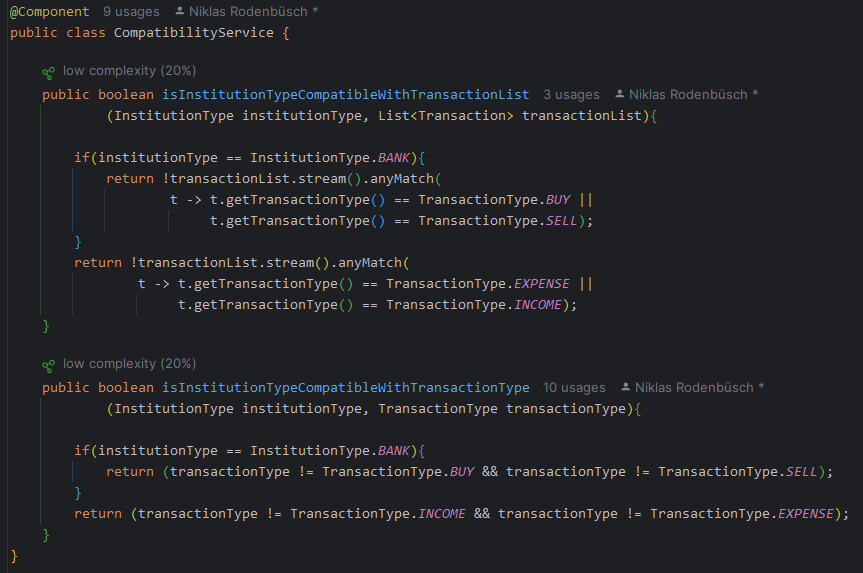
\includegraphics[width=16.5cm]{images/domainservice.png}}
    \caption[Domain Service]{Domain Service: CompatibilityService-Klasse}
    \label{fig:domainservice}
\end{figure}
\vfill